\chapter{Desarrollo de las pasantías}
\label{capitulo3}
\lhead{Capítulo 3. \emph{Diseño del sistema}}

\section{Estado del arte}
\section{Análisis de Bro}
\section{Diseño de la arquitectura del sistema}

Este capítulo tiene la intención de mostrar la visión general del modelado del sistema que se realizó a partir de las bases teóricas. Aquí, se explicará la arquitectura, el diseño y el modo en el que el IDS basado en SSM interactuará con Bro. Ademas, se detallaran las salidas y los datos de configuración
que va a considerar el sistema para su correcto funcionamiento.

\subsection{Arquitectura del sistema}

La arquitectura del detector de intrusiones que se muestra en el presente trabajo se basa en una arquitectura modular la cual está conformada por tres modulo. Un modulo para realizar la segmentación de los URIs, otro  para realizar la evaluación y un tercero para realizar el entrenamiento.

A grandes rasgos, el módulo de segmentación, se encargará de tomar los URIs previamente filtrados de las solicitudes de tipo HTTP/GET, lo normalizará y lo segmentará de la forma en la que se explicó en el apartado de ``segmentación'' de la sección \ref{sec:delimitadores}.

Por otra parte, el modulo de evaluación se encargará de evaluar la probabilidad de generación de cada uno de los segmentos del URI generados por el módulo de segmentación para al final decidir si el URI de la solicitud enviada al servidor web es anómalo o no.

Por último, el modulo de entrenamiento será el encargado de crear el modelo de normalidad del sistema. Para esto, el sistema recibirá solicitudes libres de ataques e irá calculando la probabilidad de aparición de cada una de las palabras que aparecen en las mismas.

Tanto el modulo de evaluación, como el modulo de entrenamiento son dependientes del modulo de segmentación ya que requieren de los segmentos de URI generados por eso para realizar su trabajo. 

La arquitectura del sistema queda detallada en la figura \ref{fig:arquitectura}.

\begin{figure}[tb]
\begin{center}
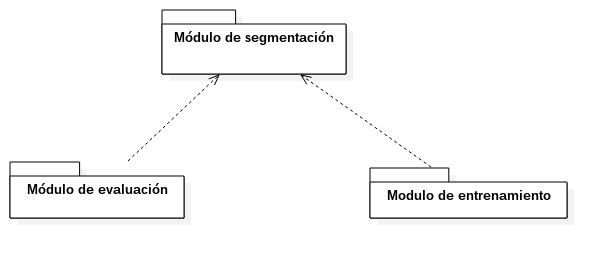
\includegraphics[width=3in]{arquitectura.png}
\caption{Arquitectura del sistema.}
\label{fig:arquitectura}
\end{center}
\end{figure}


Así mismo, es importante mencionar que el sistema contará con varios modos de operación que serán explicados a continuación:

\begin{itemize}
\item Modo evaluación: En este modo de operación solo se activarán los módulos de segmentación y evaluación del sistema. A manera general, esta modalidad, se encargará de recibir los URI previamente extraídos de las peticiones de tipo HTTP/GET, segmentarlos a tráves del módulo de segmentación, para luego evaluar si el mismo es anómalo o no
haciendo uso del módulo de evaluación. El funcionamiento de esta modalidad queda detallado en la figura \ref{fig:modoSistema}.
\item Modo entrenamiento ``Online'': En este modo de operación solo trabajaran los módulos de segmentación y entrenamiento. En esta modalidad el módulo de entrenamiento tomará los segmentos arrojados por el módulo de segmentación, calculará la probabilidad de aparición de los mismos para de esta manera ir modificando un modelo de normalidad previamente establecido. El funcionamiento de esta modalidad queda
detallado en la figura \ref{fig:modoSistema}.
\item Modo entrenamiento ``Offline'': Esta modalidad del sistema en análoga al modo de entrenamiento ``Online''. El único aspecto que diferencia a ambas modalidades es que cuando el sistema funciona en modo ``Offline'' no se toma en cuenta, ni se modifica un modelo de normalidad previamente construido. La salida de este modo de entrenamiento sera un modelo de normalidad construido desde cero.El funcionamiento de esta modalidad queda detallado en la figura \ref{fig:modoSistema}.
\end{itemize}

\begin{figure}[tb]
\begin{center}
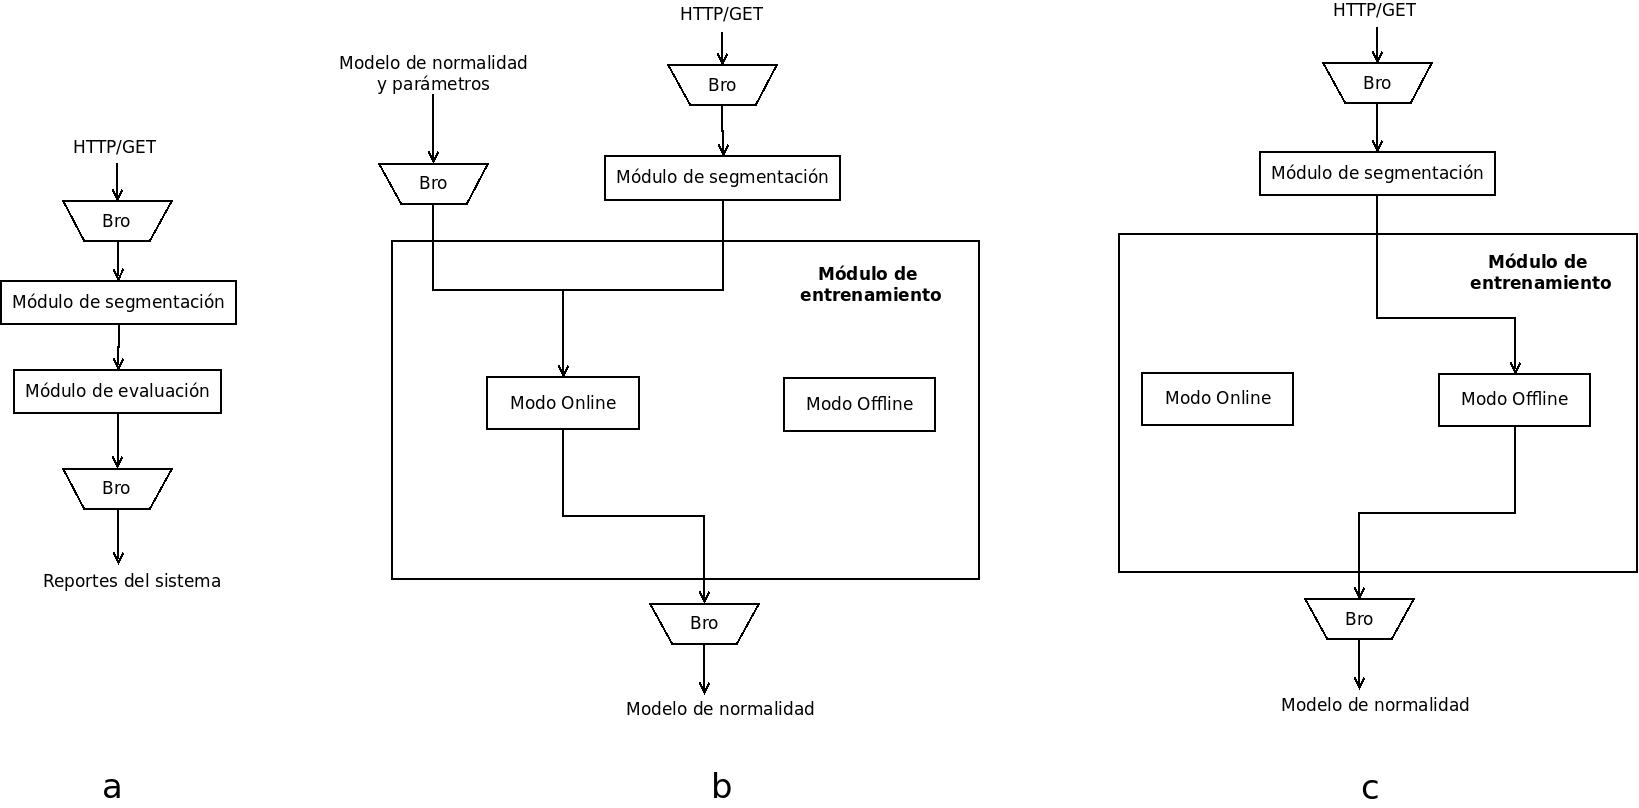
\includegraphics[width=\linewidth]{modoOperacion.jpeg}
\caption{Modo evaluación (a), modo entrenamiento ``Online'' (b), modo entrenamiento ``Offline'' (c).}
\label{fig:modoSistema}
\end{center}
\end{figure}


\subsection{Filtrado de paquetes HTTP/GET}

Esta funcionalidad se encargará de observar los paquetes de la red y filtrar aquellos de tipo HTTP/GET. Una vez obtenido este tipo de paquetes, esta función extraerá el URI adjunto al mismo.

\subsection{Módulos}

En esta sección se describirán las tareas de cada uno de los módulos que conformar la arquitectura detallada en la figura \ref{fig:arquitectura}, el modo en el que se subdividieron dichas tareas, los datos de entrada y salida, y la interacción que existe entre los mismos.

\subsubsection{Módulo de segmentación}

El modulo de segmentación es un elemento clave dentro de la construcción del IDS basado en SSM, es por eso que su buen diseño e implementación es importante para el buen funcionamiento del sistema. Este se encarga, como se mencionó anteriormente,de tomar el URI que proviene de la solicitud de tipo HTTP/GET que se le hace al servidor HTTP capturado por Bro, normalizarlo y segmentarlo siguiendo las especificaciones que se explicaron en la sección \ref{sec:delimitadores}. 

Es evidente entonces, que este modulo consta de dos funcionalidades fundamentales: la normalización de los URIs y la segmentación.  La normalización se encargará de tomar el URI de las peticiones HTTP/GET entrantes y codificarlo a formato UTF-8. Normalizar es un paso importante dentro del sistema  ya que se estandarizar la forma en las que están escritos los URIs facilita tanto la evaluación como el entrenamiento en el sistema. Por otra parte, la salida arrojada por esta función de normalización será tomada por la de segmentación, quien a su vez se encargará de segmentar el URI de la forma en la que se explica en la sección \ref{sec:delimitadores}, es decir, el URI se dividirá en las diferentes partes estipuladas en el RFC 3986: el ``host'', la ruta, los argumentos, los valores y el ``fragment''.

 En las base teórica, la segmentación de los URIs se realiza mediante un autómata que se encarga de reconocer (realizar un análisis sintáctico) y evaluar en cada uno de sus estados la probabilidad de generación de cada uno de los segmentos.  No obstante, en la función de segmentación del sistema implementado, esta tarea se modeló mediante un analizador sintáctico que hace uso de una gramática (libre de contexto) de atributos que genera el mismo lenguaje que reconoce el autómata presentado en la figura ~\ref{fig:automata}, es decir, el lenguaje de los URI.

En la figura \ref{fig:arquiSegmentacion} se puede apreciar el diagrama de bloques que refleja el funcionamiento del módulo de segmentación.

\begin{figure}[tb]
\begin{center}
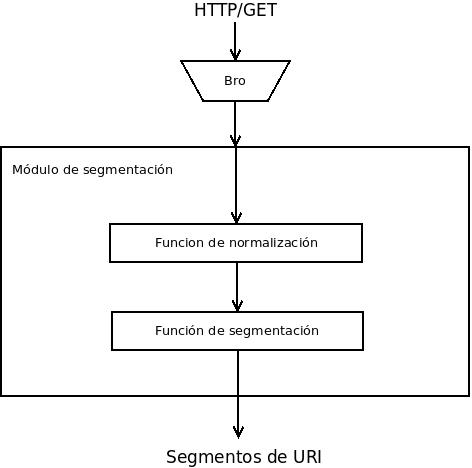
\includegraphics[width=3in]{segArquiCompleta.jpeg}
\caption{Diagrama de bloques del módulo de segmentación.}
\label{fig:arquiSegmentacion}
\end{center}
\end{figure}

\subsubsection{Módulo de evaluación}
\label{sec:evaluacion}

El módulo de evaluación, es el encargado de evaluar la probabilidad de generación de cada uno de los segmentos del URI otorgados por el modulo de segmentación, dado un modelo de normalidad. Una vez calculadas estas probabilidades, el modulo se encargará de calcular un índice de anormalidad del URI mediante el uso de las formulas descritas en la sección ~\ref{subsec:exprIndice} para luego compararlo con un parámetro $\theta$ (\ref{eq:ClaseU}) y de este modo saber si los segmentos de URI que ingresaron como entrada posee alguna anormalidad o no. Luego de realizar esta evaluación, el modulo se encargara de escribir los reportes del sistema en un ``log''.

El módulo de evaluación, está conformado por dos grandes funcionalidades: una que se encargará de leer el modelo de normalidad y  otra que calculará el índice de anormalidad y evaluará si el mismo es anómalo o no. 

El modelo teórico que fue explicado en la sección ~\ref{sec:modeloSSM} posee elementos como: un conjunto ``S'' de estados, un conjunto ``O'' de símbolos observables que se encuentran en cada estado, una matriz ``A'' que contiene la probabilidad de transición entre estados, un conjunto ``B'' de vectores que contiene la probabilidad de las palabras observadas en cada estado y un vector de probabilidades iniciales. No obstante, los únicos elementos del modelo que se necesitan ingresar en el sistema para que este funcione y realice las tareas de evaluación son: el conjunto ``O'' de símbolos observables que se encuentra en cada estado y el conjunto de vectores ``B''. El conjunto ``B'' es necesario para resolver la expresión \ref{eq:sumB}. Por otra parte, es necesario hacer uso tanto de ``B'' como ``O'' para obtener el valor de $b_{qtot}$ presentado en la ecuación \ref{eq:Pqtot}. Este elemento es sumamente importante para calcular el índice de anormalidad. Por otra parte, será necesario introducir al sistema los valores de probabilidad de fuera de vocabulario (Poov), ya que son necesarios para obtener el valor de $p_{qtot}$, presente en la ecuación \ref{eq:Pqtot}, en caso que una cadena de caracteres del URI que se esté analizando no se encuentre en el conjunto de observaciones ``O''. Además, se requiere el valor del parámetro $\theta$ para evaluar el índice de anormalidad según lo estipulado en la ecuación \ref{eq:ClaseU} .

    Entonces, en conclusión, los parámetros que requieren ser introducidos al sistema de detección de intrusiones para que este funcione de manera correcta son: el conjunto de observaciones de cada estado (O), el conjunto de vectores de probabilidad de las palabras observadas en cada estado ( $B_{S}, B_{P}, B_{A}, B_{V}$ ), los valores de probabilidad de fuera de vocabulario, es decir $P_{oovS}, P_{oovP}, P_{oovA}, P_{oovV}$ y el valor del parámetro $\theta$. Todos estos parámetros serán leídos por la función de lectura del modulo de evaluación.
    
Una vez leídos los parámetros necesarios para que el sistema funcione, estos serán enviados a la función de evaluación junto a los segmentos de URI dados por el módulo de segmentación. Una vez recibidos los datos de entrada, esta función se encargará de hallar el índice de anormalidad ($N_{s}$) mediante la expresión \ref{eq:Ns} para, de este modo compararlo con el parámetro $\theta$ como se indica en \ref{eq:ClaseU}.No obstante, las tareas de calculo y evaluación del índice de anormalidad, fueron subdivididas a su vez, en cuatro funciones. La primera de las funciones será la encargada de calcular tanto el $\varepsilon_{0}$ que aparece en la expresión \ref{eq:sumB} como la sumatoria de los logaritmos de los $p_{qtot}$ que se encuentra en \ref{eq:Ns}; la segunda función tomará el valor de $\varepsilon_{0}$ y la sumatoria de los logaritmos de los $p_{qtot}$ que calculó la primera función y procederá a efectuar todas las operaciones que hay en la expresión \ref{eq:Ns} para de este modo obtener el índice de anormalidad, $N_{s}$; por otra parte, la tercera función tendrá como tarea comparar el índice de anormalidad $N_{s}$ calculado por la tercera función, con el parámetro $\theta$ como se indica en \ref{eq:ClaseU}; la cuarta será la encargada de escribir en un archivo de texto aquellos URIs anómalos.

El diagrama de bloques presente en la figura \ref{fig:arquiEvaluacion} representa el funcionamiento del módulo de evaluación.

\begin{figure}[tb]
\begin{center}
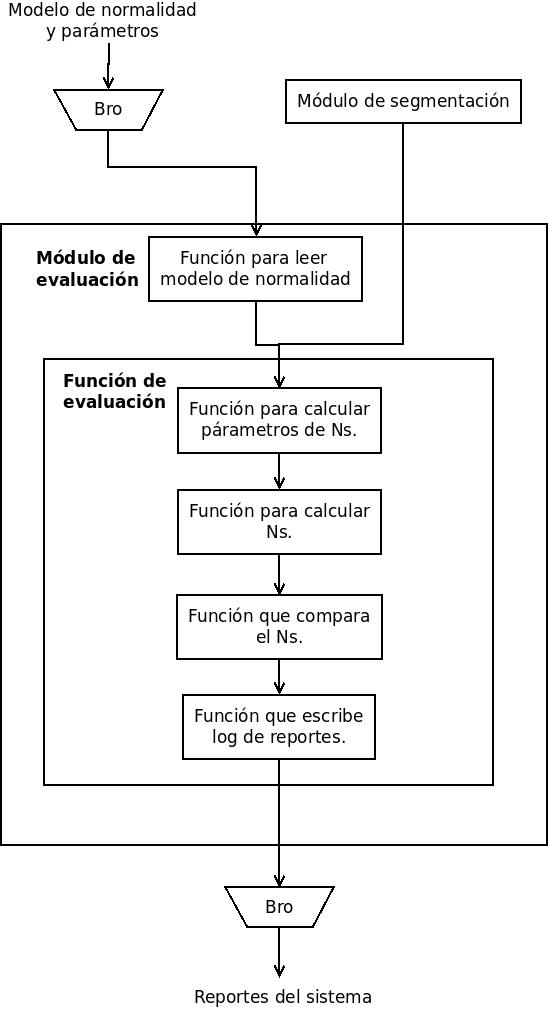
\includegraphics[width=3in]{evalArqui.jpeg}
\caption{Diagrama de bloques del módulo de evaluación.}
\label{fig:arquiEvaluacion}
\end{center}
\end{figure}

\subsubsection{Módulo de entrenamiento}\label{sec:entrenamiento}

El modelo de normalidad es uno de los aspecto importantes dentro del IDS basado en SSM ya que a partir de la información que este almacena se podrá decidir si un URI es anómalo o no dependiendo de la similitud que posea este con los datos que almacena el modelo. Por esta razón, realizar un modelo de normalidad apropiado es un aspecto  importante para que el módulo de evaluación haga detecciones de intrusiones más certeras.

El módulo encargado de elaborar los modelos de normalidad será el módulo de entrenamiento. A grandes rasgos, este se encargará de recibir un conjunto de segmentos libres de ataques proporcionados por el módulo de segmentación para ir calculando la probabilidad de aparición de cada una de las palabras que aparecen en los mismos, para finalmente, escribir en un archivo toda la información recolectada, es decir, el conjunto de palabras observadas mientras se hacía el entrenamiento, sus probabilidades de aparición y el estado del autómata en el que se observaron las mismas.

Este módulo consta de dos modos: el modo ``Offline'' y el modo ``Online''. La  diferencia fundamental entre el modo ``Online'' y el ``Offline'' es que en el primero necesita como entrada un modelo de normalidad ya construido y los segmentos de URI proporcionados por el módulo de segmentación. Una vez realizado el entrenamiento, esta modalidad se encargará de actualizar el modelo que se leyó al inicio. Por otra parte, el modo ``Online'' solo requiere como entrada los segmentos de URI y como salida proporcionará un  modelo de normalidad construido desde cero.

El modo de entrenamiento ``Offline'' fue dividido en tres funciones. La primera función irá observando los segmentos de los URIs de las peticiones que van llegando y contará el numero de veces que cada segmento fue observado durante el entrenamiento. La segunda función, toma el resultado de las observaciones realizadas por la primera función y calculará la probabilidad de aparición de cada uno de los segmentos haciendo uso de la formula \ref{eq:entrenamiento}. La tercera función tomara los resultados otorgados por la segunda función y los escribirá en un archivo de texto. Este archivo representara el modelo de normalidad construido.

Por otra parte, las tareas a realizar por el modo de entrenamiento ``Online'' fueron divididas de igual modo en tres funciones: La primera función se encargara de leer el modelo de normalidad; la segunda se encargará de tomar el modelo de normalidad leído por la primera función y el conjunto de segmentos de URI del módulo de segmentación. Esta información sera utilizada por la misma para ir calculando la probabilidad de aparición de los segmentos observados. La tercera función se encargara de recibir los resultados obtenidos por la segunda función y actualizara el modelo de normalidad previamente existente.

En la figura {fig:arquiEntrenamiento} se puede apreciar el diagrama de bloques que describe el funcionamiento del módulo de entrenamiento.

\begin{figure}[tb]
\begin{center}
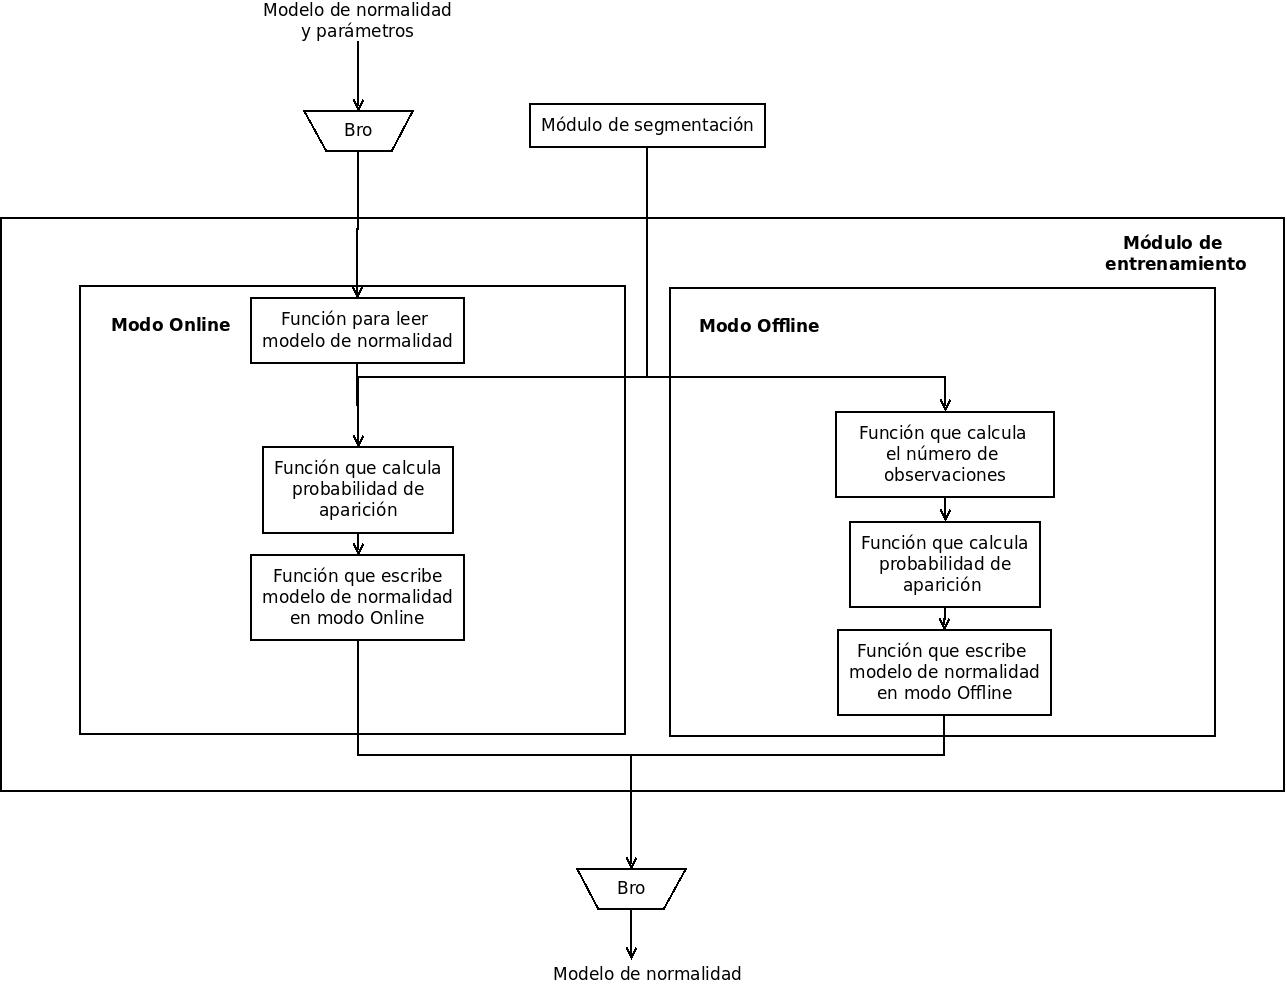
\includegraphics[width=4in]{entrenamArqui.jpeg}
\caption{Diagrama de bloques del módulo de entrenamiento.}
\label{fig:arquiEntrenamiento}
\end{center}
\end{figure}

\section{Implementación del sistema}

Una vez descrita la arquitectura modular del sistema y las funcionalidades asociadas a los diferentes componentes del sistema, en este capítulo se detallarán las cuestiones más relevantes en cuanto a su implementación.
Así, en primer lugar, se describirán como se implementó el filtro de paquetes HTTP/GET, para luego explicar las estructuras de datos utilizadas por cada uno de los módulos; los parámetros de entrada, salida y la implementación de las funciones que los componen.

\subsection{Filtrado de paquetes HTTP/GET}

El módulo de segmentación requiere como entrada los URIs extraidos de las peticiones de tipo HTTP/GET. Esta tarea se realizó haciendo uso de las herramientas brindadas por Bro. En concreto, esta funcionalidad fué implementada con un evento primitivo de Bro llamado ``http request''. Este evento se genera y almacena la información de paquetes HTTP cuando son percibidos por dicha herramienta en la red. Su formato es el siguiente:

\textbf{http request}(c: \textbf{connection}, method: \textbf{string}, original\_URI: \textbf{string},
unescaped\_URI: \textbf{string}, version: \textbf{string})

donde:

\begin{itemize}
\item c: es una estructura de datos de tipo ``connection'' que almacena de manera desglosada la información del mensaje HTTP.
\item method: Es el método extraído de la petición (e.g., GET,POST).
\item original\_URI : URI extraído de la petición (sin decodificar).
\item unescaped\_URI : URI extraído de la petición con todas las codificaciones de porcentaje decodificadas.
\item version: Número de la version HTTP (e.g. 1.1). Este estará especificado en la petición.
\end{itemize}

\subsection{Implementación del modulo de segmentación}

En esta sección, se explicará de manera detallada la implementación del módulo de segmentación y las estructuras de datos utilizadas en el mismo. Este módulo forma parte de los tres que conforman el sistema de detección de intrusiones basado en SSM.

\subsubsection{Normalización}
\label{sssec:estructuraNormalizacion}

La estructura de datos utilizada en la función de normalización es un hash table que contiene los elementos de un encoding table de tipo UTF-8, en donde las claves de la tabla serían los elementos de tipo UTF-8 y los atributos de las mismas corresponderían a los caracteres sin alguna codificación. Con esta tabla, se quiere implementar un diccionario que mapee los elementos de tipo UTF-8 con sus respectivos caracteres lo mas rapido posible.

Se utilizó un hash table para implementar este diccionario debido a que es ampliamente conocido que este tipo de tablas propocionan mucha eficiencia en el tiempo de búsqueda de sus elementos.

Para implementar este tipo de estructura se utilizó el tipo de dato ``table'' otorgado por el lenguaje de scripting de Bro.

\subsubsection{Función de segmentación}
\label{sssec:estructuraSegmentacion}

Por otra parte, la estructura de datos utilizada en la función de segmentación de este módulo es un registro en el cual se almacenan todos los segmentos que se originan a partir de la segmentación de un URI, el URI sin segmentar, un booleano que informa si el URI segmentado sigue con la sintaxis establecida en el RFC 3896, y el número de estados que fueron visitados en el autómata presentado en el modelo teórico.
 
Se escogió un registro para almacenar la información ya que el lenguaje de ``scripting'' de Bro solo presenta como alternativa el tipo de dato ``record'' para crear un tipo de dato compuesto. 

El registro creado esta conformado por los siguientes campos:
\begin{itemize}
\item uri: Es una variable de tipo ``string'' que almacena el URI sin segmentar. Este campo del registro será utilizado por el módulo de entrenamiento al momento de escribir los logs correspondientes.
\item host: Es una variable de tipo ``hash table'' cuyas claves son número y sus valores  son de tipo string. En esta sección se almacenan los segmentos del URI correspondiente al host.
\item path: Es una variable de tipo ``hash table'' cuyas claves son número y sus valores  son de tipo string. En esta sección se almacenan los segmentos del URI correspondiente al path.
\item query: Es una variable de tipo ``hash table'' cuyas claves y sus valores son de tipo string. En esta sección se almacenan los atributos y los valores del query del URI en caso de que el mismo posea. Los atributos y los valores se almacenarán en una hash table como se mencionó con anterioridad, en donde la clave del mismo serán los atributos del query y en donde los valores de las misma serán los valores del query del URI.
\item fragment: Es una variable de tipo ``string'' que almacenará el fragment del URI en caso de poseerlo.
\item número de estados: es una variable de tipo entero que almacena el número de estados del autómata que se emplea en el módelo teórico fueron visitados para reconocer el URI. Este campo del registro será utilizado por el módulo de evaluación.
\item uri correcto: es una variable de tipo booleano que indica si el URI está sintácticamente correcto o no.
\end{itemize}

El nombre que recibirá este tipo de estructura es ``UriSegmentado''. La misma se puede apreciar gráficamente en la figura (INSERTE REFERENCIA).

Además de utilizar el tipo de dato ``UriSegmentado'', el módulo de segmentación hace uso de una estructura de datos compuesta, primitiva del lenguaje de ``scripting'' de Bro llamada  ``URI''. Dicha estructura posee los siguientes campos:

\begin{itemize}
\item scheme: Es un campo opcional de tipo ``string'' que almacena el protocolo del URI.

\item netlocation: Es un campo de tipo ``string'' que almacena el nombre de dominio o la dirección IP del URI.

\item portnum: Es un campo opcional de tipo ``count''  que almacena el número de puerto del URI.
\item path:Es un campo de tipo ``string'' que almacena la ruta del URI.

\item file\_name: En un campo opcional de tipo ``string'' que almacena el nombre completo  del archivo de la ruta del URI junto a su extensión.

\item file\_base: En un campo opcional de tipo ``string'' que almacena el nombre  del archivo de la ruta del URI sin su extensión.

\item file\_ext: En un campo opcional de tipo ``string'' que almacena la extensión del archivo de la ruta.

\item params: Es un campo opcional de tipo ``table'' que almacena todos los parámetros de la consulta del URI. Esta tabla mapea todos los atributos con sus valores.

\end{itemize}

La estructura ``URI'' se puede apreciar gráficamente en la figura (INSERTE NUMERO DE LA FIGURA).

\subsection{Función de segmentación}

En la función de segmentación, el problema que se quiere resolver es el siguiente:construir un analizador sintáctico que haga uso de una gramática (libre de contexto) de atributos que genera el mismo lenguaje que reconoce el autómata presentado en la figura 2.4. A nivel de implementación lo que se quiere construir es un analizador sintáctico que verifique que los URIs tengan una estructura sintáctica correcta según los estándares del RFC 3986, y que a la vez vaya almacenando los segmentos, delimitados por los delimitadores presentados en la sección 2.6, en la estructura de datos de la figura 4.2,
detallada en la sección 4.2.1.

A continuación se presentara la forma en que se modeló y se implementó el problema presentado con anterioridad haciendo uso de las herramientas presentadas por el lenguaje de ``scripting'' de Bro.

Para realizar el analizador sintáctico se requiere construir una gramática libre de contexto.

Antes de presentar la gramática se mostrarán los tokens que utilizará la misma como elementos terminales.

Estos tokens utilizarán las expresiones regulares que soporta Bro. Estas están basadas en las expresiones regulares empleadas en Lex, la librería para realizar análisis léxicos del lenguaje de programación C. Estos tokens utilizarán las expresiones regulares que soporta Bro. Estas están basadas en
las expresiones regulares empleadas en Lex, la librería para realizar análisis léxicos del lenguaje de programación C.
La lista de tokens utiliza es la siguiente:

\begin{itemize}
\item protocolo: “http”|”https”
\item host: $(([a-z]+[a-z0-9\-]*[.])?([a-z0-9]+[a-z0-9\-]*[.])+[a-z]{2,3}|localhost)(:([0-9]{1,5}))?|$\\ ((25[0-5]|2[0-4][0-9]|[01]?[0-9][0-9]?)\.){3}(25[0-5]|2[0-4][0-9]|[01]?[0-9][0-9]?)(:([0-9]{1,5}))?
\item elementoPath: [\^?\#]*
\item atributo: [\^\#\&=]
\item valor: [\^\#\&]
\item fragmento: (\#.*)
\end{itemize}

Por otra parte, la gramática libre de contexto en la que está basada la función de análisis sintáctico es la siguiente.

\begin{equation}\label{eq:gramatica}
\begin{aligned}
S -> protocolo “ :// ” H  \\
H -> host “/” P | host \\
P -> P’ “?” Q | P’ “\#” F | P’ \\
Q -> Q’ “\#“ F | Q’ \\
F -> fragment \\
P’ -> \lambda \\
P’ ->  elementoPath \\
P’ -> elementoPath “/” P’ \\
Q’ -> atributo “=” valor \\
Q’ -> atributo “=” valor “\&” Q’ \\
\end{aligned}
\end{equation}

Donde, el elemento de inicio de esta gramática es el símbolo no terminal ``S''

Para almacenar los segmentos en la estructura de datos compuesta de tipo ``uriSegmentado'' que se presentó en la sección ~\ref{sssec:estructuraSegmentacion} a la gramática \ref{eq:gramatica} se le van a asociar atributos a algunas de las reglas de la misma. A este tipo de gramática se le llama gramática de atributos. Los atributos de dicha gramática serán escritos en el lenguaje de scripting de Bro.

\begin{equation}\label{eq:gramaticaAtributos}
\begin{aligned}
S -> protocolo “ :// ” H { uri\$protocolo := protocolo } \\
H -> host “/” P | host { uri\$host := host  } \\
P -> P’ “?” Q | P’ “\#” F | P’ \\
Q -> Q’ “\#“ F | Q’ \\
F -> fragment { uri\$fragment := fragment } \\
P’ -> \lambda  { uri\$path.append(“”) } \\
P’ ->  elementoPath { uri\$path.append(elementoPath) } \\
P’ -> elementoPath “/” P’ { uri\$path.append(elementoPath) } \\
Q’ -> atributo “=” valor { uri\$query[atributo] := valor } \\
Q’ -> atributo “=” valor “\&” Q’ { uri\$query[atributo] := valor } \\
\end{aligned}
\end{equation}

    La gramática de atributos presentada \ref{eq:gramaticaAtributos} representa el modelo de lo que se implementó haciendo uso de Bro.

    Como Bro no cuenta con una librería propia para programar un parser de manera sencilla, se hizo uso de las herramientas con las que cuenta este para procesar cadena de caracteres y expresiones regulares. Las funciones fundamentales que se utilizaron para implementar  la gramática \ref{eq:gramaticaAtributos} fueron: ``split'', ``split\_all'' y ``decompose\_uri''.

A continuación se explicara un poco el funcionamiento de cada una de ellas.

\begin{itemize}
\item split:
La función ``split'' tiene la siguiente forma
\textbf{split}(str: \textbf{string}, re: \textbf{pattern}) : \textbf{string\_array Attributes:\&deprecated}

Esta función se encarga de dividir una cadena de caracteres de acuerdo a un patrón e introduce el resultado en un arreglo. Por ejemplo, $split"a-b--cd", /(\-)+/)$ retorna $\{"a", "b", "cd"\}.$

Los parámetros de dicha función son:

\begin{itemize}
\item Str:La cadena de caracteres que se quiere dividir. 
\item Re: El patrón que describe lo delimitadores mediante los cuales será dividida la cadena de caracteres. 
\item Retorna: Un arreglo de caracteres donde cada elemento corresponde a una subcadena de caracteres de Str separado por Re.
\end{itemize}

\item split\_all():
Esta función realiza el mismo trabajo que ``split'' con la diferencia que los separadores son incluidos también el parámetro de salida.  Por ejemplo, $split\_all("a-b--cd", /(\-)+/)$ retorna $\{"a", "-", "b", "--", "cd"\}$.

\item decompose\_uri:
La función decompose\_uri tiene la siguiente forma: \textbf{decompose\_uri}(uri: \textbf{string}) : \textbf{URI}

decompose\_uri dado un URI, retorna una estructura de datos compuesta de tipo URI explicada en la sección ~\ref{sssec:estructuraSegmentacion} que contiene información como el protocolo,la ruta, el número de puerto y los parámetros de las consultas del URI recibido.
\end{itemize}

Por otra parte, para implementar la gramática ~\ref{eq:gramaticaAtributos} se modelaron los elementos no finales de la misma como funciones. Por otra parte, los elementos finales, fueron extraídos haciendo uso de ``split'' y ``split\_all''.

En conclusión, la función encargada de segmentar y realizar el análisis sintáctico del módulo de segmentación posee la siguiente estructura:

\textbf{segmentar}(uri: \textbf{string}) : \textbf{UriSegmentado}.
La función se encargará, de tomar una cadena de caracteres y segmentarla según delimitados por los delimitadores presentados en la sección 2.6 y almacenar los mismo en la estructura ``UriSegmentado''.

Los parámetros de dicha función son:

\begin{itemize}
\item url : Cadena de caracteres que será segmentada.
\end{itemize}

\section{Evaluación y pruebas}
